\section{Terrorist Relationships as a Social Network?}
\label{sec:Terrorist Relationships as a Social Network?}
In this section, the proprieties of the terrorist relationships line graph as a relational network is explored. As~\cite{ZSG2006} mentions, an organisation needs interpersonal connection to function and studying the structure of the social organisation could yield valuable insight.

\cite{krawczyk_line_2011}~found that on the basis of a study of an online social network, a social network could be well approximated by the line graph of a scale free network. If that propriety can be verified by our dataset, %then we could gain information from the original graph from which the line graph originates.

Social sciences studies have shown that social/relationship networks have the particularities of homophily and transitivity.
Logically if $a$ \& $b$ are friends and $c$\& $b$ are also, the it is more likely that $a$ \& $c$ are friends than not. This mathematically translates to:
\begin{equation}
	a \sim b \text{ and } b \sim c \text{ then } a \sim c
\end{equation}

As a first research question we will try to verify that our dataset derives from a scale-free network, implying that the graph that generated the relationship dataset have proprieties similar to social networks.
By creating a scale-free network and making its line graph, we compared the degree distribution of the relationship dataset we were able to show that.

\begin{figure}[H]
\begin{center}
    \begin{subfigure}[b]{0.45\textwidth}
        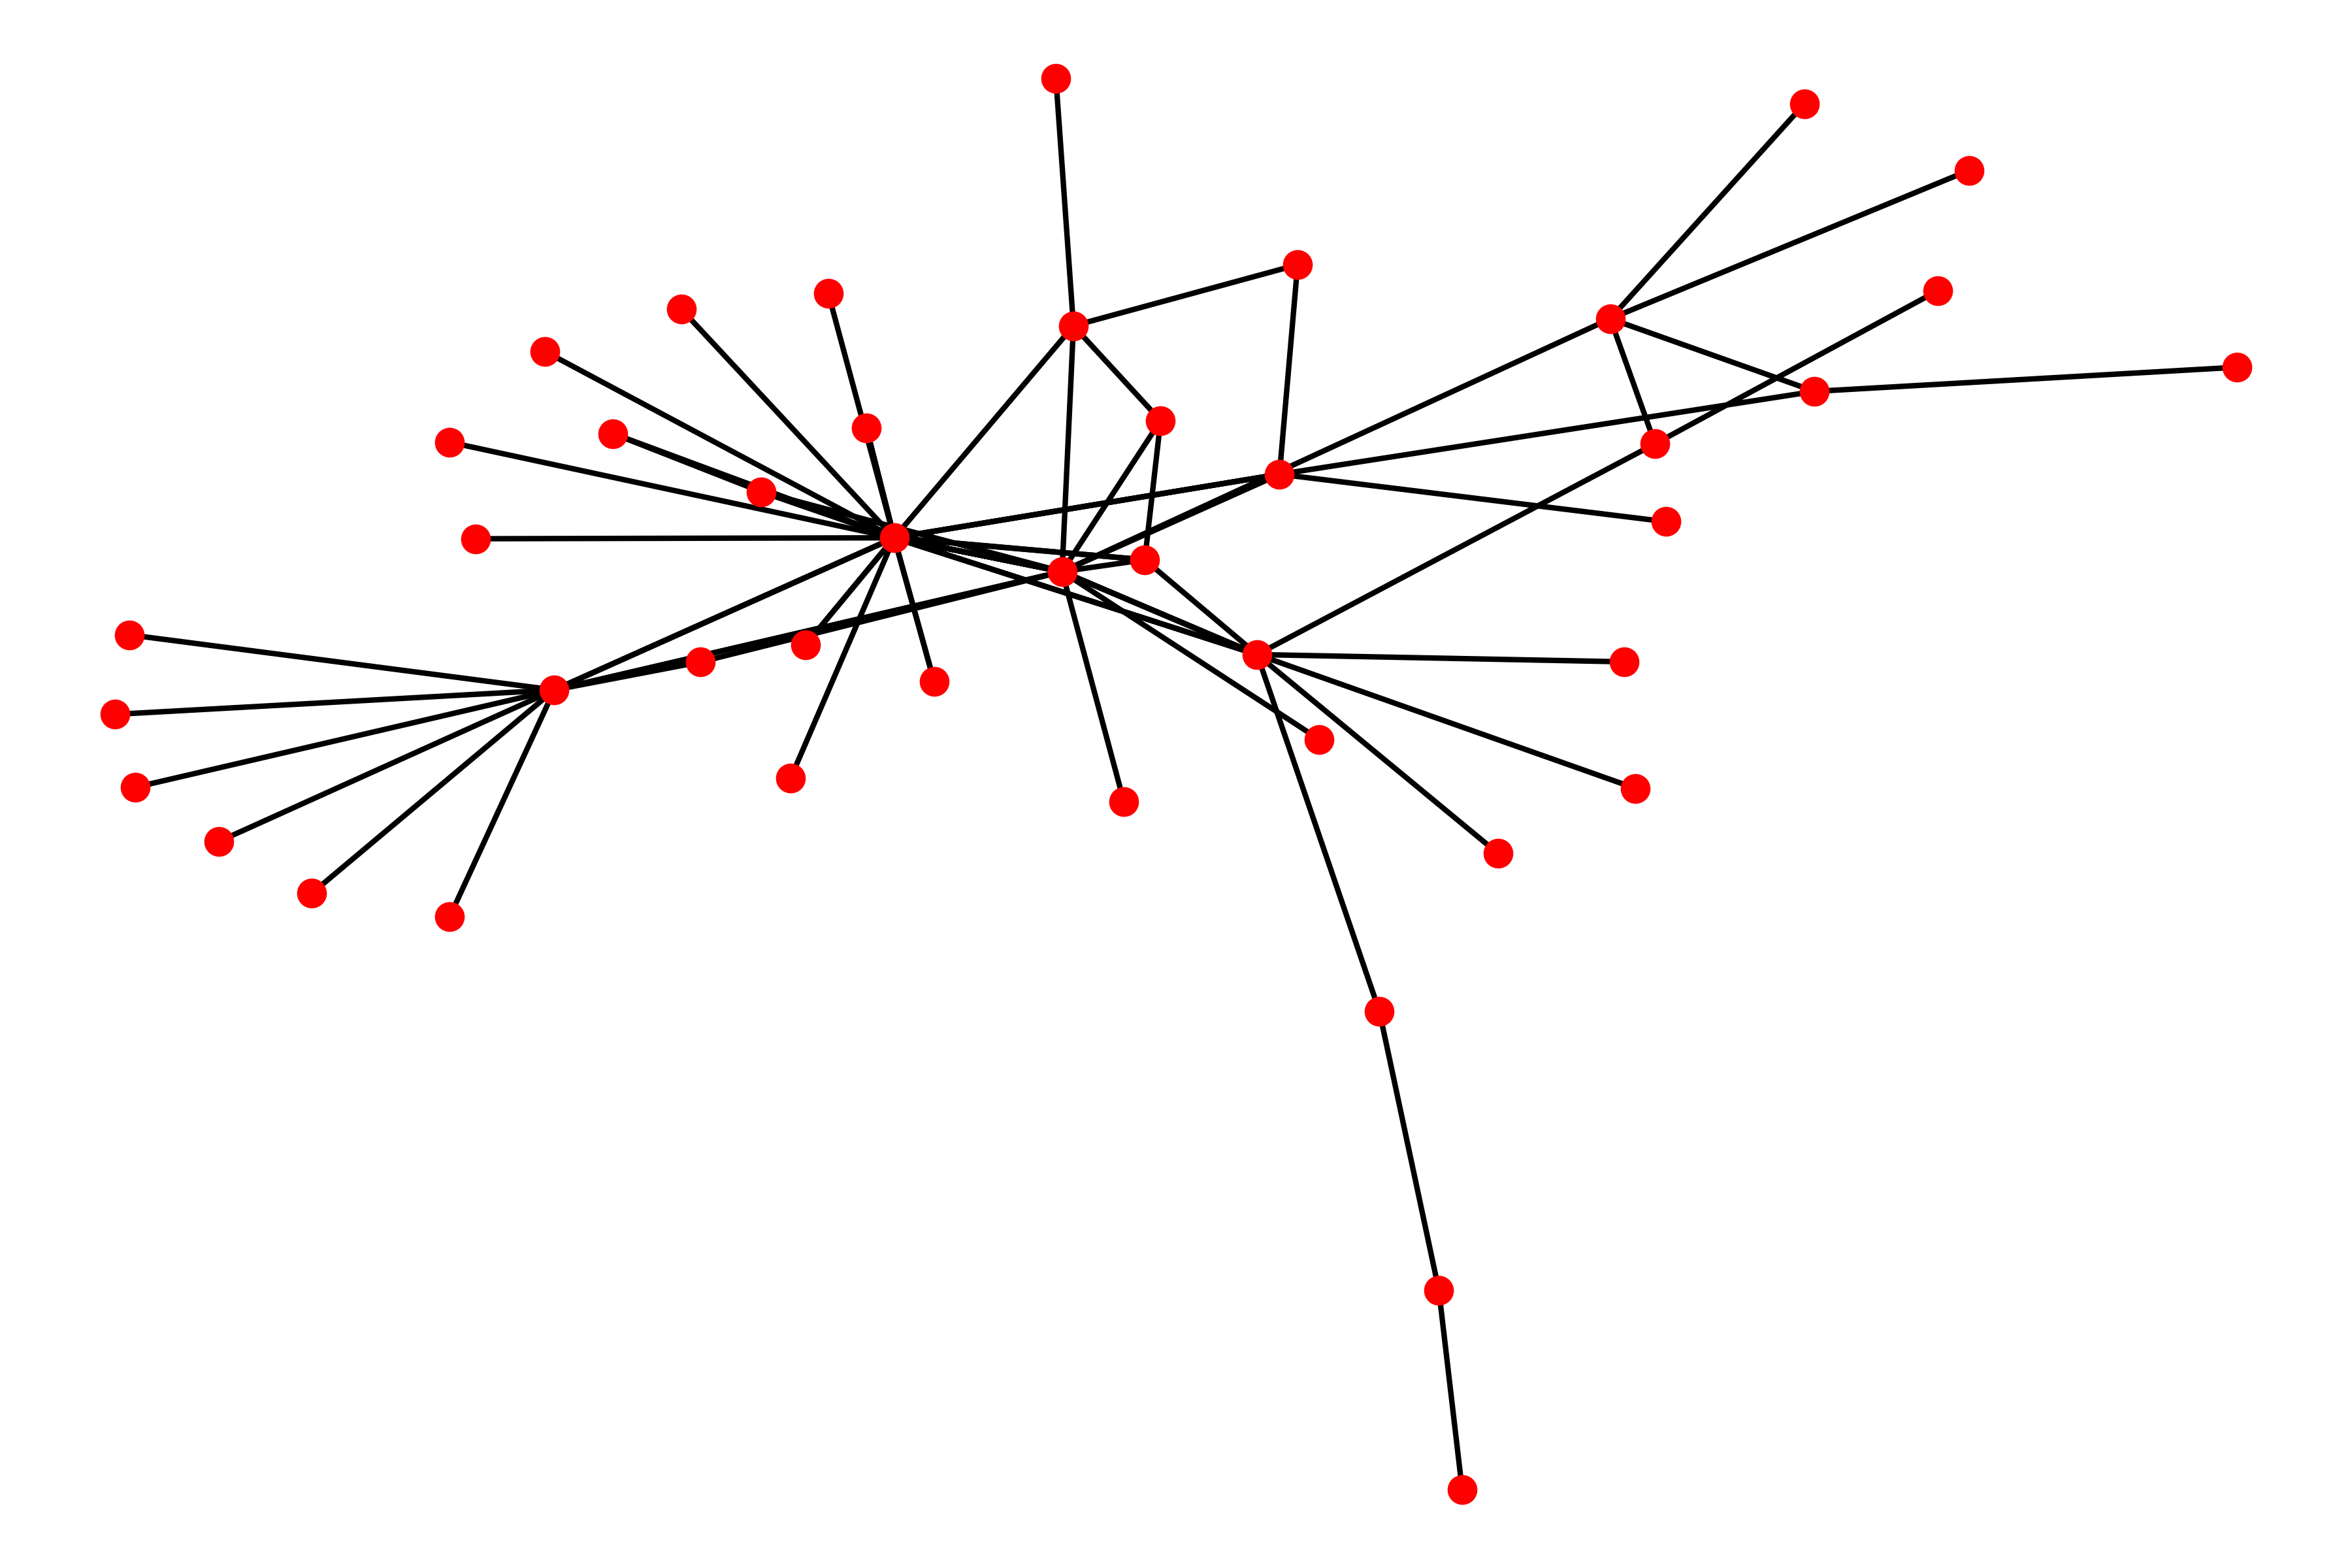
\includegraphics[width=\textwidth]{graphScaleFree.png}
        \caption{Scale free network}
        \label{fig:Scalefree}
    \end{subfigure}
    ~
    \begin{subfigure}[b]{0.45\textwidth}
        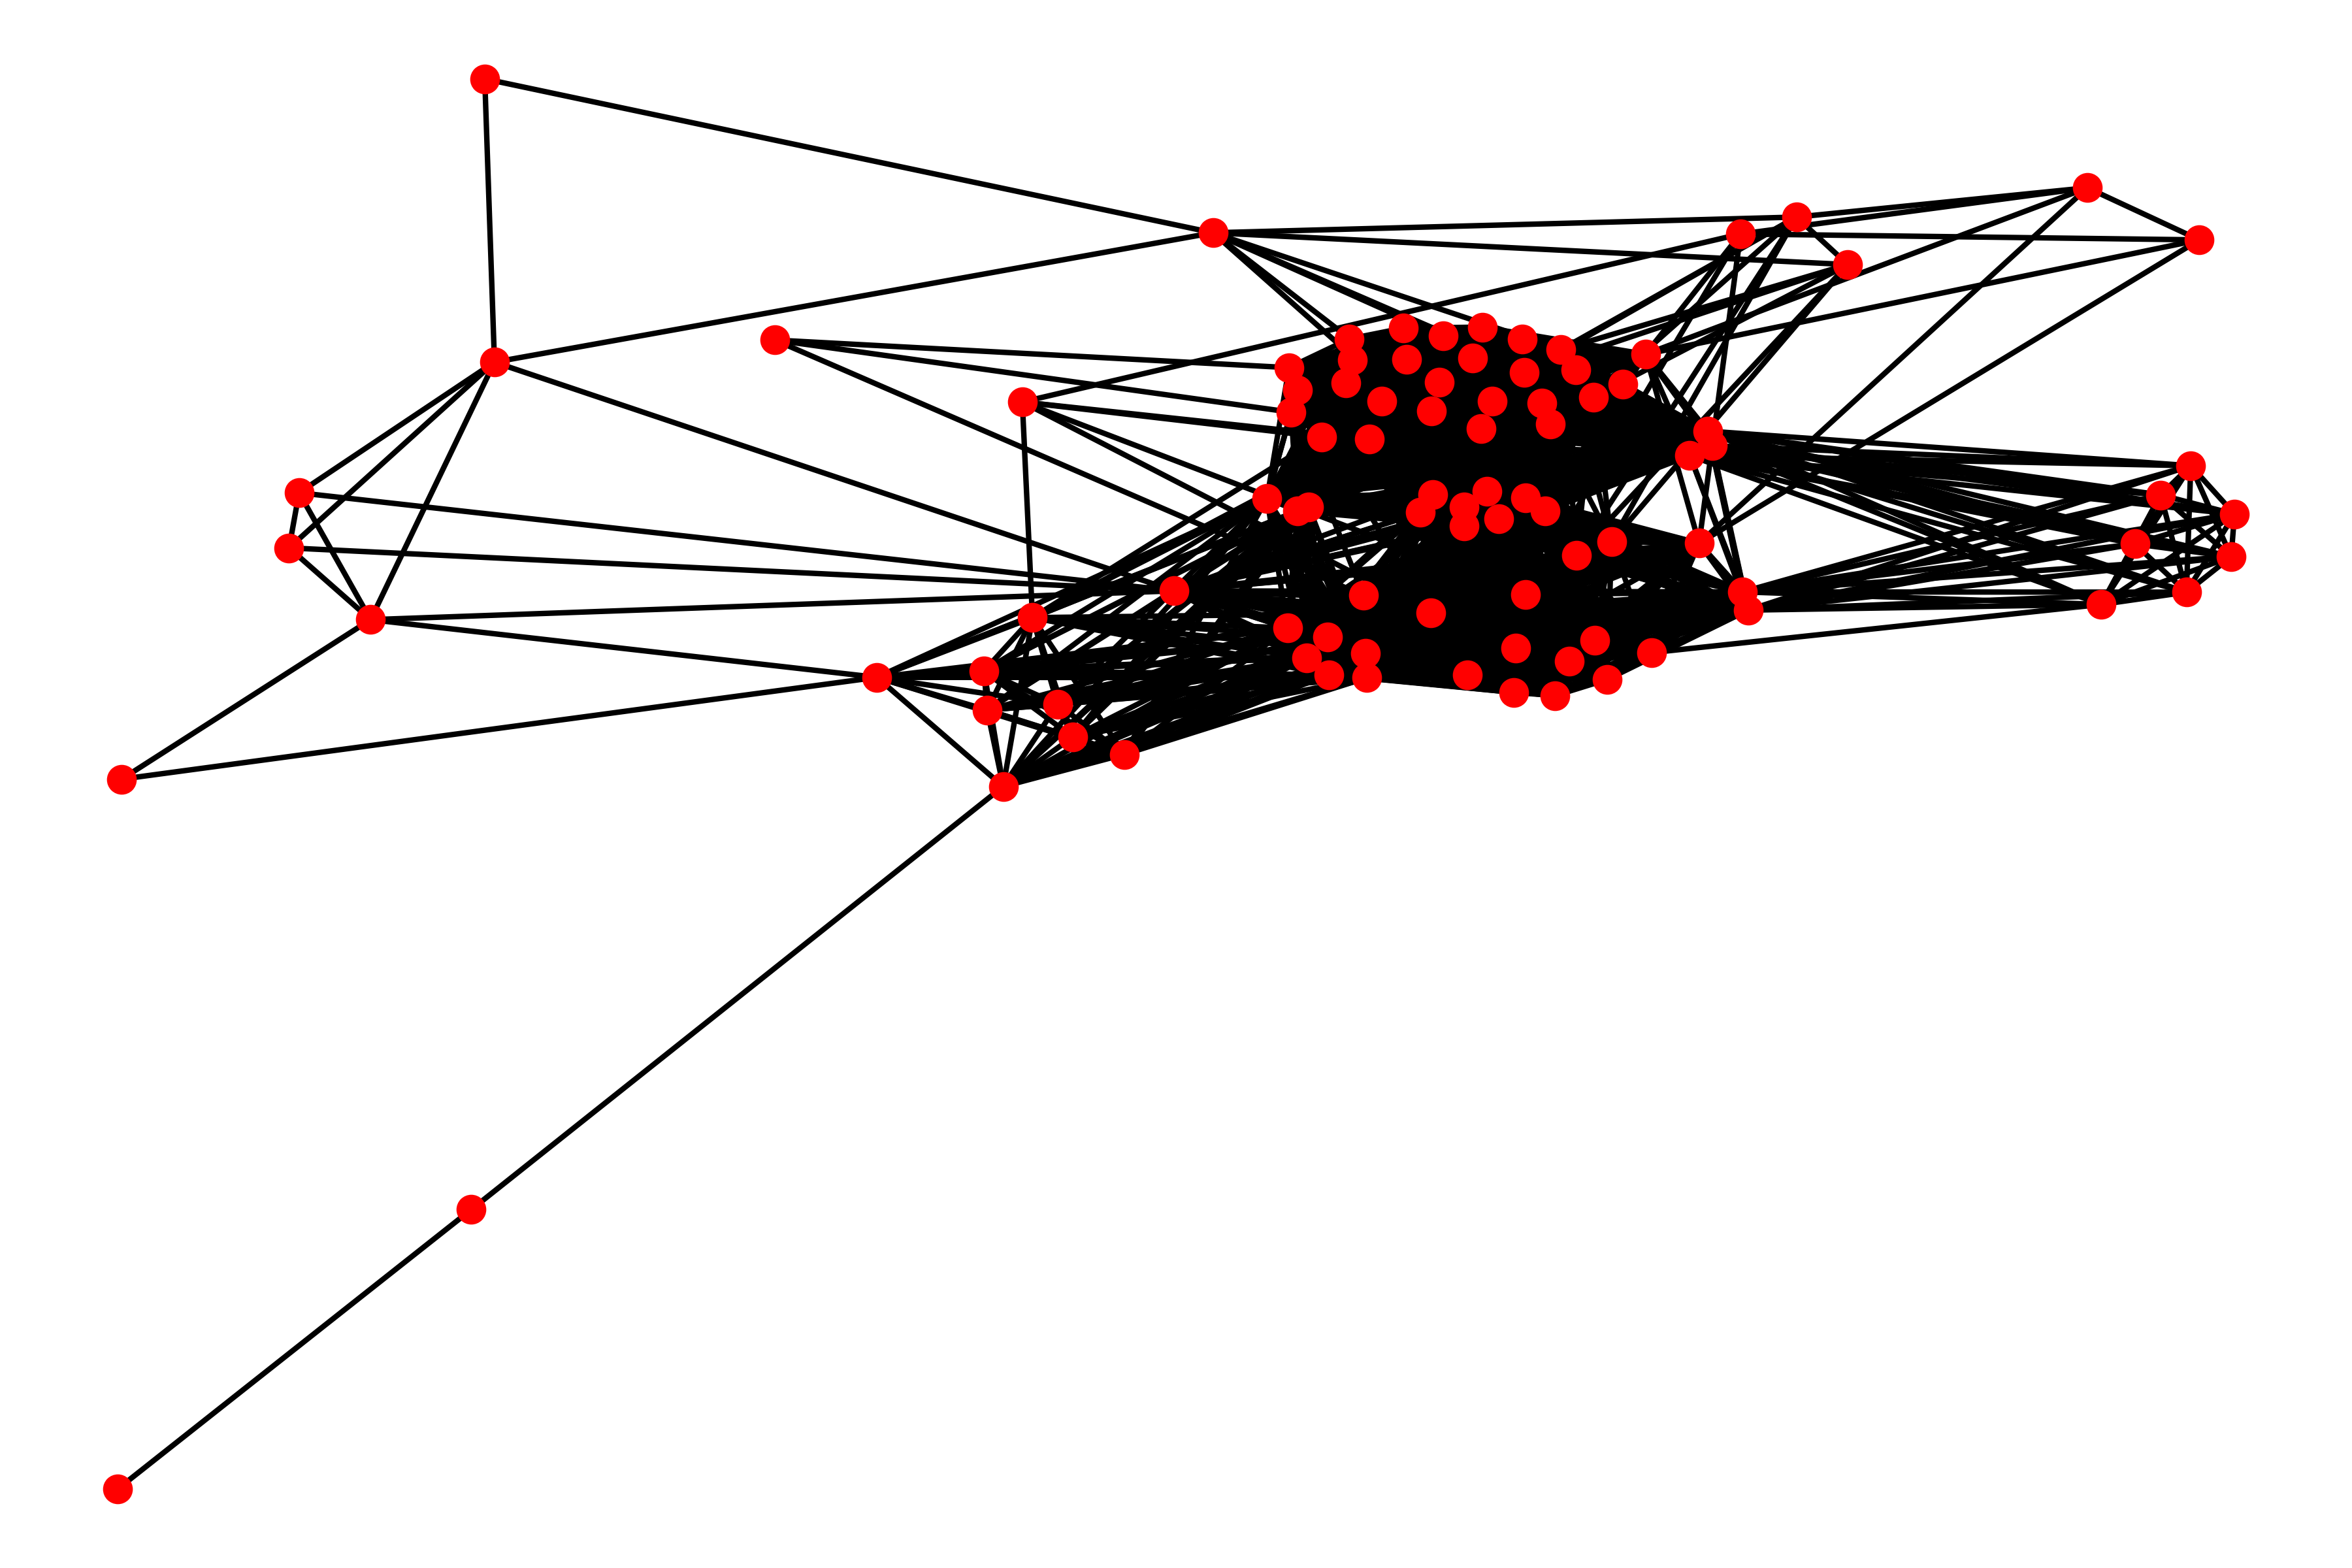
\includegraphics[width=\textwidth]{graphLineScaleFree.png}
        \caption{Line graph of scale free network}
        \label{fig:lineG}
    \end{subfigure}
    
    \begin{subfigure}[b]{\textwidth}
    	\begin{centering}
        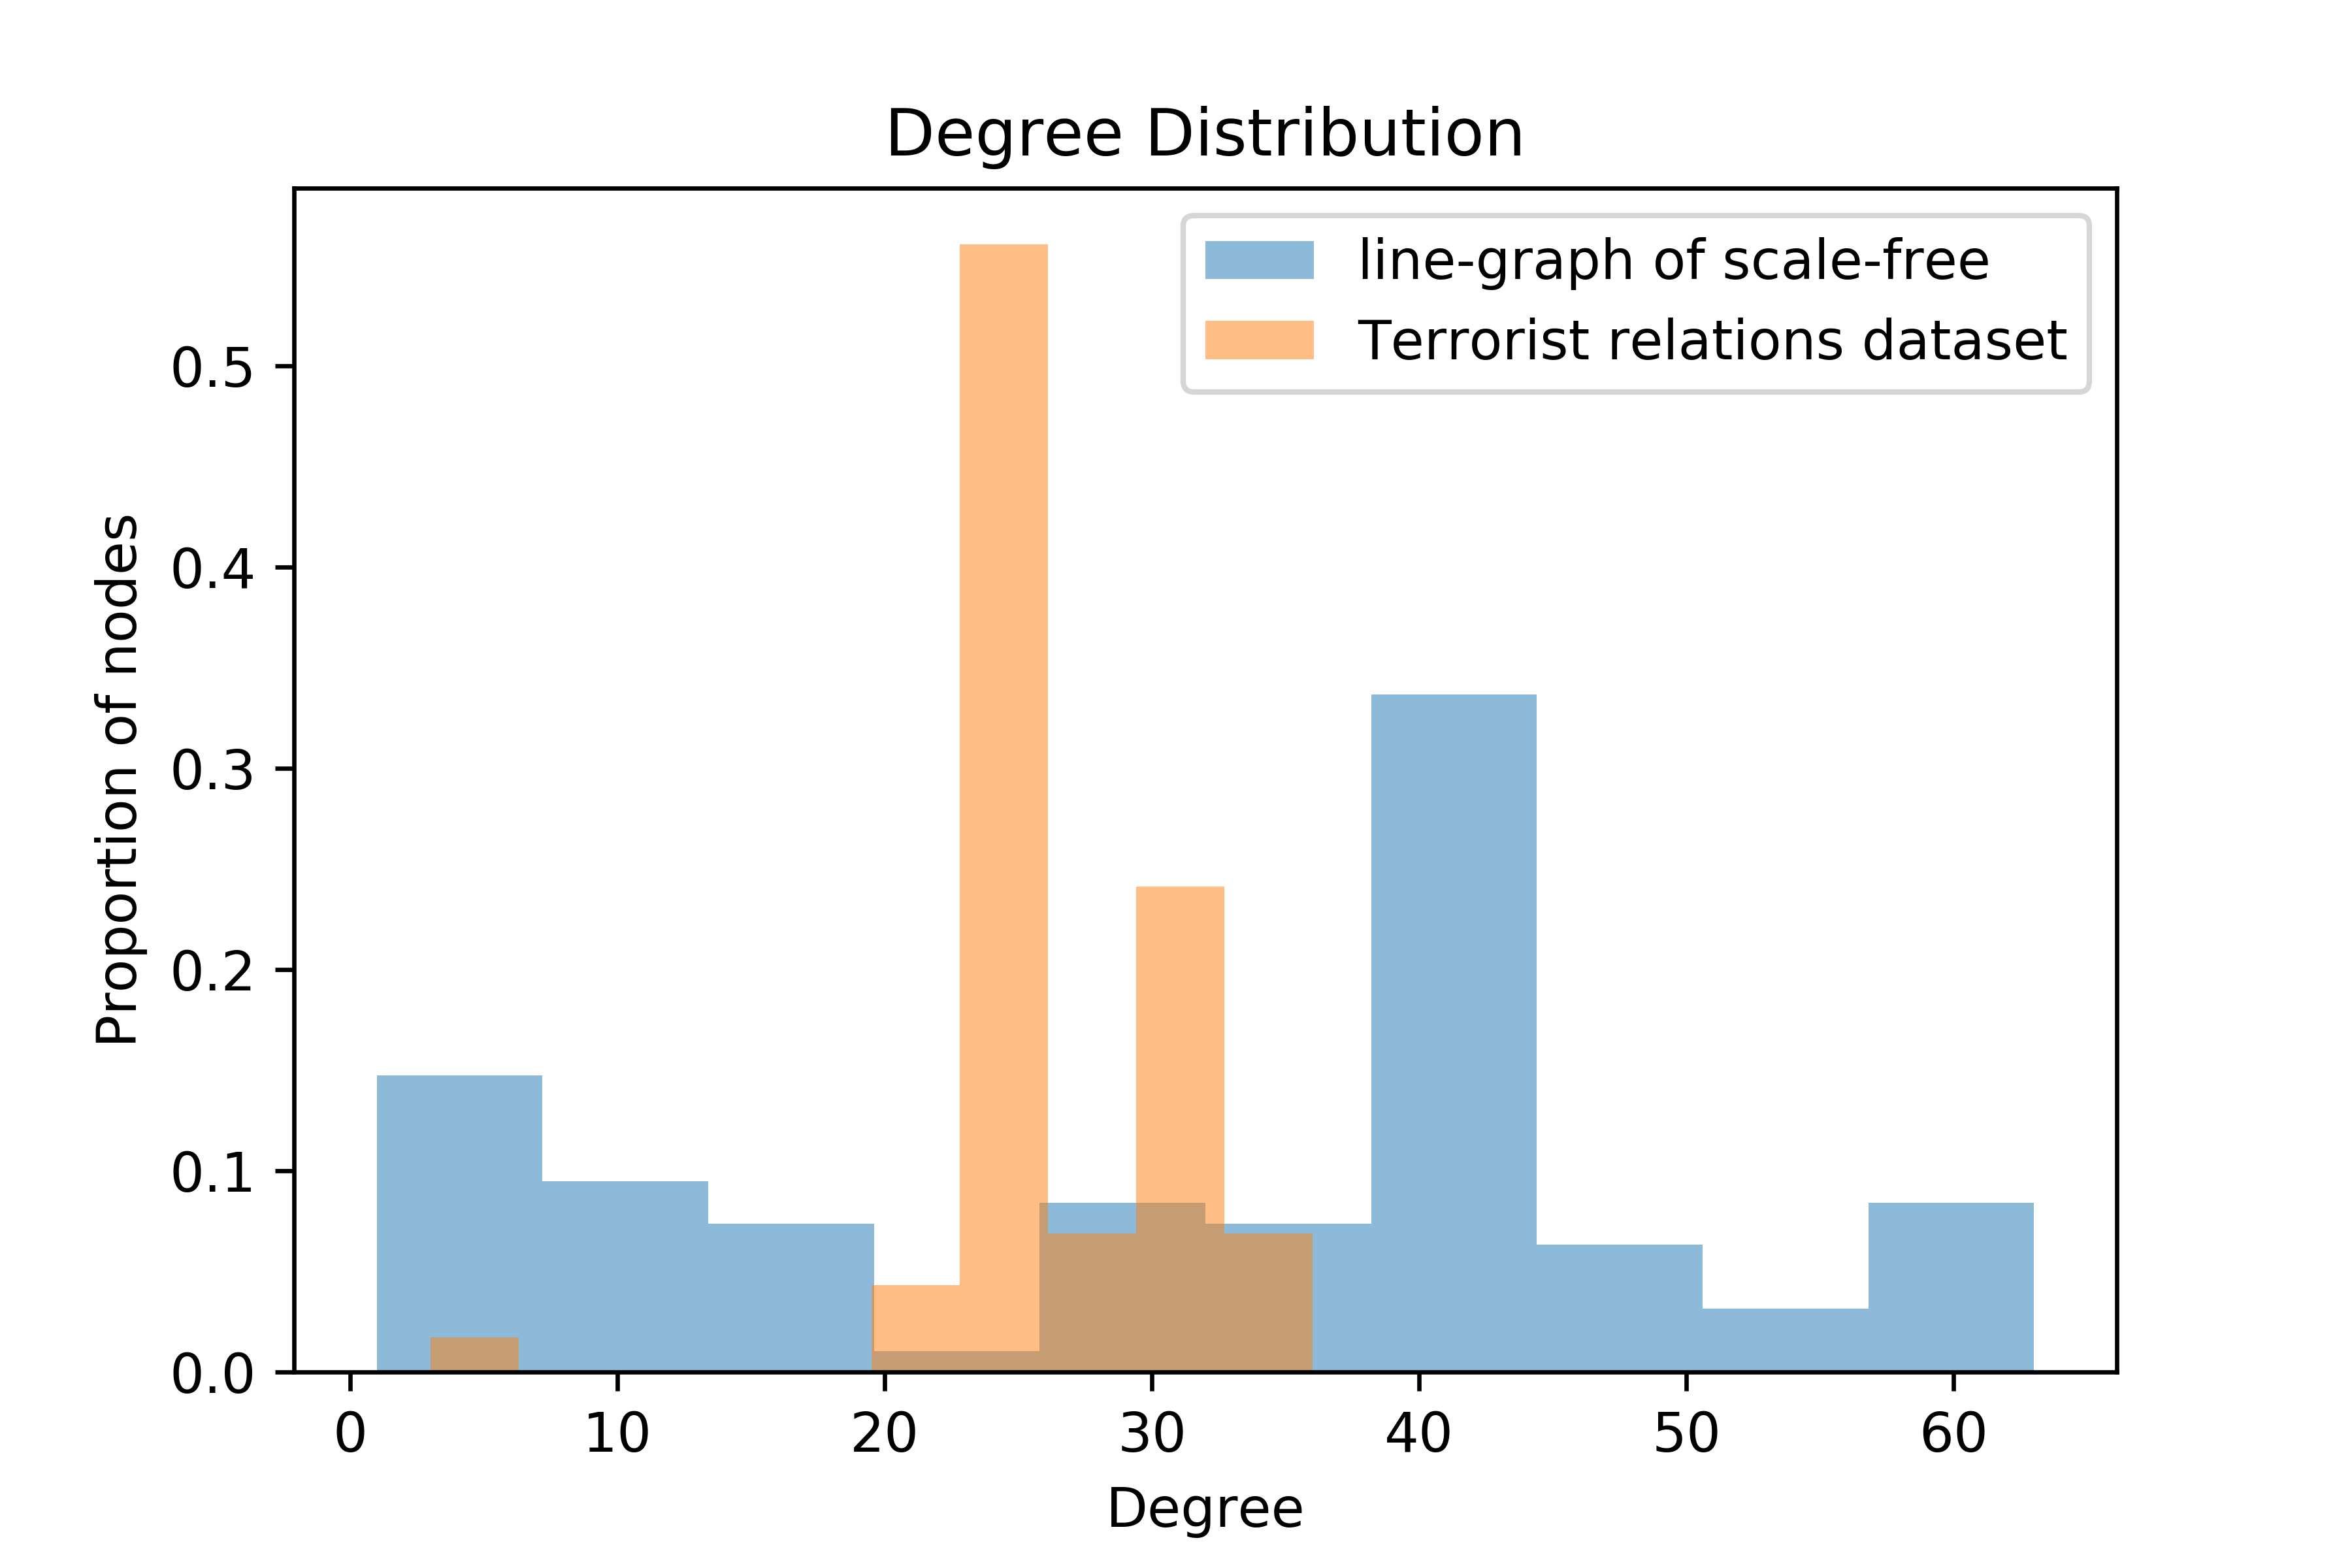
\includegraphics[width=.5\textwidth]{DegreeDiff.png}
        \caption{\centering Comparison of the degree distribution of the two line graphs. In blue, the created line graph and in orange the degrees of the relationships graph}
        \label{fig:DegDiff}
        \end{centering}
    \end{subfigure}
\caption{Comparison of a scale free network and the terrorist relationships network.}
\label{fig:RelationshipScaleFree}
\end{center}
\end{figure}


%\subsection{Terrorist Relations Dataset}
%
%\subsection{Terror Attacks Dataset}
%\label{subsec:terror attack quality}
